\documentclass[../ECON-281-Notes.tex]{subfiles}
\begin{document}
\chapter{Consumer Choice}

\section{Budget Line}
\begin{Definition}
    {Budget Line}
    Shows the different bundles from any two goods that the consumer can buy if they use all their income.

    The \textbf{Budget Line} has a negative slope. Since your income is fixed, to get more of one good, you must buy less from the other good.

    \[P_X \cdot X + P_Y \cdot Y = I\]
    Where \(I\) is income, \(P_X\) is the price of \(X\), \(P_Y\) is the price of \(Y\). Both \(X\) and \(Y\) are the quantities of X and Y respectively. 
\end{Definition}

\begin{Definition}
    {Budget Constraint}
    Set "group" of all feasible bundles
\end{Definition}

\begin{Definition}
    {Slope of Budget Line}
    \[\text{Slope of budget line} =  -\frac{P_X}{P_Y}\]
    Note that the budget line is \emph{negative}.
\end{Definition}

\subsection{Shifts in the B.L}
If Income, or the price of X and Y changes by the same percentage then the shift is parallel. A increase in I, or a decrease in both prices by the same \% will lead to a rightward shift. While a decrease in I, or a increase in both prices by the same \% will lead to a leftward shift.

If both income and both prices increases by the same \% then the budget line stays the same. 

If the price of one good increases then the budget line's intercept will change along the axis of that good (X or Y). A decrease in price will move the intercept away from the origin while a increase in price will move the intercept towards the origin.

\section{Consumer Equilibrium}
The main objective of a consumer is to maximize their utility with their budget. 

\begin{Definition}
    {Interior Solution}
    Consumer buys a combination of both X and Y.
\end{Definition}

The consumer's expenditure minimization problem results in the same optimal basket as the consumer's utility maximization problem if the required level of utility for the expenditure minimizer is the same as the maximized utility for the utility maximizer.

\begin{figure}[htbp]
    \centering
    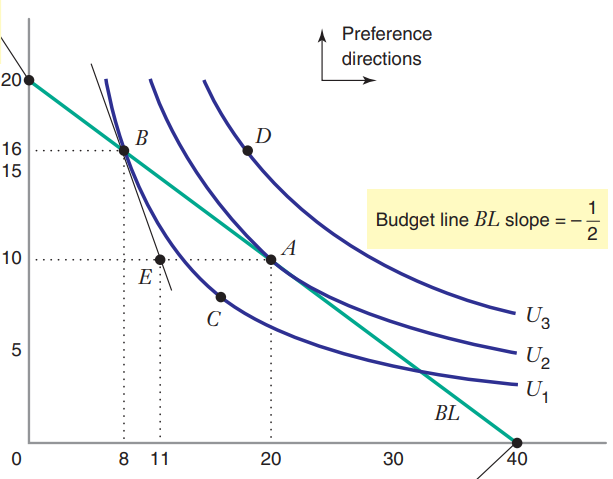
\includegraphics[width=0.8\columnwidth]{../assets/BL-indiff-curve.png}
    \caption{Budget line with Indifference Curve}
    \label{fig:BL_ind_curve}
\end{figure}
Utility is maximized at the pint where the B.L is tangent to the indifference curve. 
That means the slope of the budget line is equal to the slope of the indifference curve 
\[
    \frac{P_X}{P_Y} = \frac{MU_X}{MU_Y} \rightarrow \frac{MU_X}{P_X} = \frac{MU_Y}{P_Y}
\]
The second equation normalizes the marginal utility with price.

Equilibrium happens when B.L is tangent to the indifference curve not when it intersect it.

In the \cref{fig:BL_ind_curve} \(B\) is feasible but only \(A\) is tangent to the highest utility indifference curve.

\subsection{Moving towards equilibrium}
Suppose that:
\[\frac{MU_X}{P_X} > \frac{MU_Y}{P_Y}\]
this means that you will get more marginal utility of X per dollar or unit of cost than Y. Therefore you would buy or consume more of X and buy or consume less of Y. This continues until
\[\frac{MU_X}{P_X} = \frac{MU_Y}{P_Y}\]


\section{Algorithms for Consumer Choice}
\subsection{Cobb-Douglas}
\begin{enumerate}
    \item Find \(MU_X\) and \(MU_Y\) by doing the derivative
    \item Find \(MRS_{XY} = \frac{MU_X}{MU_Y}\) 
    \item Find the equilibrium \(\frac{P_X}{P_Y} = \frac{MU_X}{MU_Y}\)
    \item Rearrange so you solve for X or Y
    \item Substitute that equation into the B.L
    \item Find the best quantity for the other good not used in 4.
    \item Find the best quantity for the other good not used in 6.
    \item You can find the utility value here as well.
\end{enumerate}

\subsection{Perfect Complements or Leontief}
\begin{enumerate}
    \item Isolate for X or Y from the function \(aX = bY\) from \(U = \text{min}(aX, bY)\)
    \item Substitute that equation into the B.L
    \item Find the best quantity for the other good not used in 1.
    \item Find the best quantity for the other good not used in 3.
    \item You can find the utility value here as well.
\end{enumerate}

\subsection{Perfect Substitutes or Linear}
\begin{enumerate}
    \item Find \(MU_X\) and \(MU_Y\) by doing the derivative
    \item \(\frac{MU_X}{P_X}\) and \(\frac{MU_Y}{P_Y}\)
    \item If \(\frac{MU_X}{P_X} > \frac{MU_Y}{P_Y}\) buy only X \(X = \frac{I}{P_X}\)
    \item If \(\frac{MU_X}{P_X} < \frac{MU_Y}{P_Y}\) buy only Y \(Y = \frac{I}{P_Y}\)
    \item If \(\frac{MU_X}{P_X} = \frac{MU_Y}{P_Y}\) buy any 
    \item From here you can get the maximum utility.
\end{enumerate}

\section{Derivation of Demand Function}
The demand function is in the form \[X = \frac{I}{aP_X}\] or \[Y = \frac{I}{aP_Y}\]

\subsection{Income normal or inferior}
To determine if a good is normal or inferior one just needs to find the sign of the derivative of the demand function \(\frac{\partial X}{\partial I}\) or
\(\frac{\partial Y}{\partial I}\). If the sign is \textbf{Positive} then the good is normal if \textbf{Negative} then the good is inferior.

\subsection{Substitutes or Complements}
To determine if a good is a substitute or a complement of another good you can replace \(I\) with \(P_Y\) \(\frac{\partial X}{\partial P_Y}\) or \(P_X\) \(\frac{\partial Y}{\partial P_X}\). If the sign is \textbf{Positive} then the goods are substitutes if they are \textbf{Negative} the goods are complements. If they are 0 then the goods are unrelated.

\subsection{Demand Curve in Case of Corner Solution}
For the corner solution case the demand curves are of a piecewise function.

Let 
\[A = \frac{MU_X\cdot P_Y}{MU_Y}\] 
and 
\[B = \frac{MU_Y\cdot P_X}{MU_X}\]

\[ Q\cdot d_X = 
\begin{cases} 
    0 & P_X > A \\
    \frac{I}{P_X} & P_X < A
\end{cases}
\]
\[ Q\cdot d_Y = 
\begin{cases} 
    0 & P_Y > B \\
    \frac{I}{P_Y} & P_Y < B
\end{cases}
\]

\section{Composite Good}
So far we assumed we have 2 goods X and Y. Now we will introduce a new type of good which is called \textbf{Composite Good} which is the expenditure on all other goods. 

\begin{DndSidebar}[color=PhbLightGreen]{Price of Composite Good}
    The price of a composite good is \textbf{alaways} 1. 
\end{DndSidebar}

\section{Application of Consumer Choice}

\subsection{Joining a Club}
Enables the consumer to buy the good or service at a discounted rate after paying for a flat fee membership.

\subsubsection{Determining if it's worth it}
You find the budget line with and without the membership remembering to take out the cost of the membership from \(I\) for the membership B.L.
Check the slopes of the two B.L and you can determine if the membership is worth it to the consumer.

\begin{figure}[htbp]
    \centering
    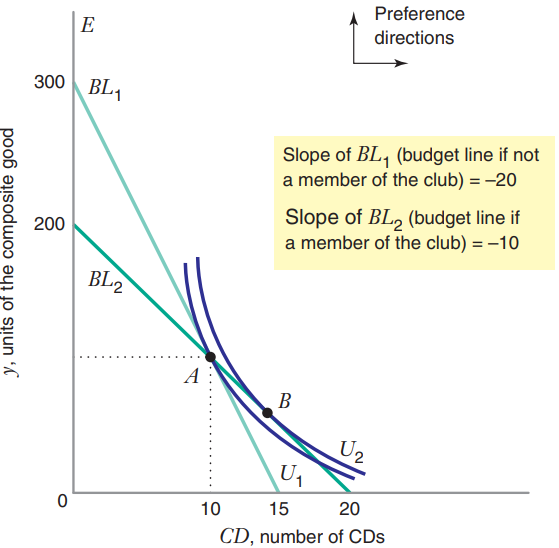
\includegraphics[width=0.8\columnwidth]{../assets/joining_a_club.png}
    \caption{BL Joining a Club}
    \label{fig:BL_join_club}
\end{figure}

\subsection{Calling Plans}
For this you have a fixed free amount of minutes from the plan and each additional minutes after cost a certain amount. 

Find the B.L for both and compare and contrast between the two.
\begin{figure}[htbp]
    \centering
    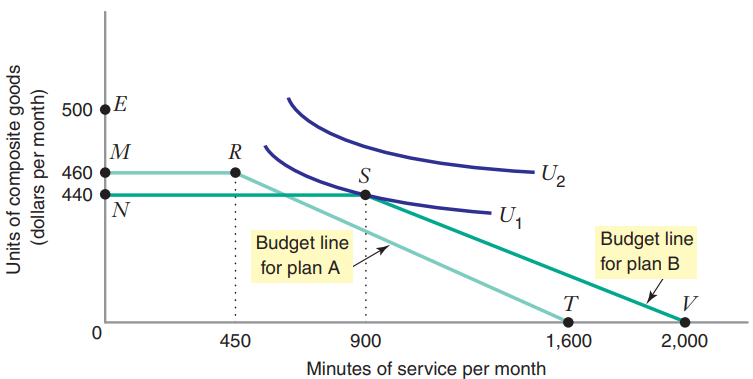
\includegraphics[width=0.8\columnwidth]{../assets/cellphone_plan.png}
    \caption{ML Cellphone plan}
    \label{fig:BL_cell_plan}
\end{figure}
it may or may not be worth it depending on where the ind. curve is.
\newpage
\subsection{Quantity Discount}
This is where the BL has a kink in the middle where after a certain amount the cost of buying more is less per unit. 

Find the B.L for both and compare and contrast between the two.

\begin{Note}
    The budget line before the discount kink is the same. It only chances after the quantity that applies the discount.
\end{Note}

\begin{figure}[!h]
    \centering
    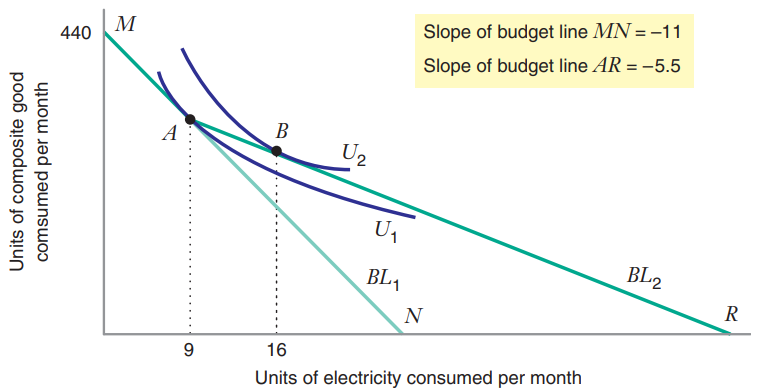
\includegraphics[width=0.8\columnwidth]{../assets/quantity_discount.png}
    \caption{BL Quantity Discount}
    \label{fig:BL_quant_dis}
\end{figure}
\end{document}
